\documentclass[10pt,a4paper]{article}

% --- Page Geometry ---
\usepackage[margin=1.8cm,top=2.2cm,bottom=2.2cm,headheight=15pt]{geometry}

% --- Typography & Encodings ---
\usepackage[T1]{fontenc}
\usepackage[utf8]{inputenc}
\usepackage{lmodern}
\usepackage{microtype}

% --- Math Packages ---
\usepackage{amsmath,amssymb,amsfonts}

% --- Tables & Arrays ---
\usepackage{booktabs}
\usepackage{tabularx}
\usepackage{longtable}
\usepackage{array}
\usepackage{multirow}
\usepackage{makecell}

% --- Colors ---
\usepackage{xcolor}
\definecolor{NavyBlue}{RGB}{16, 44, 87}
\definecolor{DarkTeal}{RGB}{0, 90, 112}
\definecolor{SlateGray}{RGB}{60, 64, 67}
\definecolor{LightGray}{RGB}{246, 248, 250}
\definecolor{BorderGray}{RGB}{209, 213, 218}
\definecolor{AccentGreen}{RGB}{24, 134, 75}
\definecolor{CodeDark}{RGB}{36, 41, 46}
\definecolor{KeywordBlue}{RGB}{0, 92, 197}
\definecolor{StringRed}{RGB}{186, 40, 34}
\definecolor{CommentGray}{RGB}{106, 115, 125}

% --- Section Styling ---
\usepackage{titlesec}
\titleformat{\section}
  {\color{NavyBlue}\Large\bfseries}
  {\thesection}{1em}{}[\titlerule]
\titleformat{\subsection}
  {\color{DarkTeal}\large\bfseries}
  {\thesubsection}{1em}{}
\titleformat{\subsubsection}
  {\color{SlateGray}\normalsize\bfseries}
  {\thesubsubsection}{1em}{}

% --- Headers & Footers ---
\usepackage{fancyhdr}
\usepackage{lastpage}
\pagestyle{fancy}
\fancyhf{}
\fancyhead[L]{\small\color{SlateGray}\textbf{BMS Firmware Reverse Engineering} --- Knowledge Base \& Technical Reference}
\fancyhead[R]{\small\color{SlateGray}\textbf{21S 70Ah NCM}}
\fancyfoot[L]{\footnotesize\color{SlateGray}Confidential / Yatri Mobility Systems --- Engineering Reference Manual}
\fancyfoot[R]{\footnotesize\color{SlateGray}Page \thepage\ of \pageref{LastPage}}
\renewcommand{\headrulewidth}{0.4pt}
\renewcommand{\footrulewidth}{0.4pt}

% --- Hyperlinks ---
\usepackage{hyperref}
\hypersetup{
    colorlinks=true,
    linkcolor=NavyBlue,
    citecolor=NavyBlue,
    filecolor=DarkTeal,
    urlcolor=DarkTeal,
    pdfauthor={Yatri BMS Reverse Engineering Team},
    pdftitle={BMS Firmware Reverse Engineering Knowledge Base},
    pdfsubject={21S 70Ah NCM BMS Technical Reference},
    pdfkeywords={BMS, N32G45x, DVC1124, NCM, SOC, OCV, CAN, Modbus, Firmware}
}

% --- Code Listings ---
\usepackage{listings}
\lstset{
    basicstyle=\ttfamily\footnotesize\color{CodeDark},
    backgroundcolor=\color{LightGray},
    frame=single,
    rulecolor=\color{BorderGray},
    breaklines=true,
    breakatwhitespace=true,
    captionpos=b,
    showstringspaces=false,
    keywordstyle=\color{KeywordBlue}\bfseries,
    stringstyle=\color{StringRed},
    commentstyle=\color{CommentGray}\itshape,
    numbers=none,
    tabsize=4,
    xleftmargin=1em,
    xrightmargin=1em,
    aboveskip=1em,
    belowskip=1em
}

% --- TikZ Diagrams ---
\usepackage{tikz}
\usetikzlibrary{shapes.geometric, arrows.meta, positioning, calc, backgrounds, fit}

\tikzset{
    box/.style={
        rectangle,
        rounded corners=3pt,
        draw=NavyBlue!80,
        fill=LightGray,
        thick,
        align=center,
        font=\sffamily\footnotesize,
        inner sep=6pt
    },
    decision/.style={
        diamond,
        aspect=2,
        draw=DarkTeal!90,
        fill=DarkTeal!10,
        thick,
        align=center,
        font=\sffamily\footnotesize,
        inner sep=4pt
    },
    arrow/.style={
        ->,
        >=Stealth,
        thick,
        color=NavyBlue!80
    },
    dashedarrow/.style={
        ->,
        >=Stealth,
        thick,
        dashed,
        color=DarkTeal!80
    },
    stagebox/.style={
        rectangle,
        rounded corners=4pt,
        draw=DarkTeal!80,
        fill=NavyBlue!5,
        thick,
        align=left,
        font=\sffamily\footnotesize,
        inner sep=7pt
    }
}

% --- Custom Environments ---
\usepackage{tcolorbox}
\tcbuselibrary{skins,breakable}

\newtcolorbox{calloutbox}[1][]{
    enhanced,
    breakable,
    colback=LightGray,
    colframe=NavyBlue!75,
    fonttitle=\bfseries\sffamily\color{NavyBlue},
    title=#1,
    arc=3pt,
    boxrule=1pt,
    left=8pt,
    right=8pt,
    top=6pt,
    bottom=6pt,
    before skip=1em,
    after skip=1em
}

\newtcolorbox{warningbox}[1][Warning]{
    enhanced,
    breakable,
    colback=red!5,
    colframe=red!70!black,
    fonttitle=\bfseries\sffamily\color{red!70!black},
    title=#1,
    arc=3pt,
    boxrule=1pt,
    left=8pt,
    right=8pt,
    top=6pt,
    bottom=6pt,
    before skip=1em,
    after skip=1em
}

% --- Document Starts ---
\begin{document}

% --- Title Block ---
\begin{titlepage}
\begin{center}
    \vspace*{1cm}
    {\Huge \bfseries \color{NavyBlue} BMS Firmware Reverse Engineering}\\[0.5cm]
    {\LARGE \bfseries \color{DarkTeal} Technical Knowledge Base \& Engineering Handbook}\\[0.8cm]
    {\large \textbf{Comprehensive Specification, Decompiled Analysis, Architecture \& C Reconstruction}}\\[1.5cm]
    
    \begin{tcolorbox}[enhanced,colback=LightGray,colframe=NavyBlue,width=0.95\textwidth,arc=4pt,boxrule=1.2pt]
    \centering
    \begin{tabular}{ll}
        \textbf{Project:} & 21S 70Ah NCM Battery Management System (Nepal EV Market) \\
        \textbf{Target MCU:} & Nations Technologies N32G45x (ARM Cortex-M4F @ 144 MHz) \\
        \textbf{Analog Front End:} & Devechip DVC1124-1 (24-Channel Precision AFE) \\
        \textbf{Firmware Container:} & \texttt{6495.004615.SPB24-DVC24-006-1010-A30.[Nepal21s70Ah].V28.DL.B72E0EEC.hex} \\
        \textbf{Flash Link Base:} & \texttt{0x08008000} (Application) / \texttt{0x08000000} (IAP Bootloader) \\
        \textbf{Last Updated:} & November 2026 \\
        \textbf{Version:} & Release V28 / Document Revision 2.4 \\
    \end{tabular}
    \end{tcolorbox}
    
    \vspace{2cm}
    \begin{calloutbox}[Executive Notice]
    This engineering manual contains the complete reverse-engineered technical specifications, decompiled firmware architectures, mathematical models, communication matrices, register maps, and verified clean-room C reconstructions for the 21S1P 70Ah NCM Lithium-Ion Battery Management System.
    \end{calloutbox}
    
    \vfill
    {\small \color{SlateGray} Yatri Mobility Systems --- Battery Systems Research \& Firmware Engineering Group}
\end{center}
\end{titlepage}

\tableofcontents
\newpage

% ==============================================================================
\section{Executive Summary \& Purpose}
% ==============================================================================
This Knowledge Base serves as the primary technical reference and engineering handbook for the reverse engineering, firmware reconstruction, and feature extension of the 21S 70Ah NCM Battery Management System (BMS) deployed in electric vehicle powertrains.

The original vendor delivery package consists of a closed, proprietary ASCII-hex container targeting the Nations Technologies N32G45x ARM Cortex-M4F microcontroller coupled to the Devechip DVC1124-1 24-channel Analog Front End (AFE). This handbook comprehensively details:
\begin{enumerate}
    \item \textbf{Container Extraction \& Dual Verification:} Cryptographic CRC32 and arithmetic byte-sum algorithms verifying binary integrity.
    \item \textbf{Microcontroller \& Hardware Architecture:} Memory maps, NVIC vectors, bit-banged and peripheral bus configurations, and board pinouts.
    \item \textbf{AFE Deep Register Architecture:} Complete 24-register map, scaling factors, hardware comparator protections, and 3-phase interleaved cell balancing.
    \item \textbf{Core State Machine \& Protection Engine:} Interlocking safety rules, pre-charge contactor sequencing, body-diode thermal bypass, and RTC low-power sleep modes.
    \item \textbf{State of Health (SOH) \& Capacity Learning:} Mathematical degradation models, 2D dynamic discharge and charge C-rate matrices, and quiescent self-discharge tracking.
    \item \textbf{Hybrid SOC Estimator:} Dual-mode Coulomb integration under dynamic load fused with 2D chemical Open-Circuit Voltage (OCV) recalibration at rest.
    \item \textbf{Communication Matrices:} 29-bit extended CAN 2.0B protocol, Modbus RTU register layouts, and proprietary PC upper-computer diagnostic frames.
    \item \textbf{Non-Volatile Storage \& Black-Box Logger:} AT24Cxx EEPROM layouts, on-chip Flash driver, MCU 96-bit UID anti-cloning lock, and 32-byte rolling fault snapshots with root-cause diagnostic indexes.
    \item \textbf{Safe Field Updating on Sealed Packs:} A 100\% non-destructive code-cave trampoline architecture allowing custom C logic execution over CAN without endangering bootloader recovery.
\end{enumerate}

% ==============================================================================
\section{End-to-End Reverse Engineering Workflow}
% ==============================================================================
The extraction pipeline transitions systematically from an opaque vendor delivery container to a fully verifiable, compilable, host-testable C repository.

\begin{figure}[htbp]
\centering
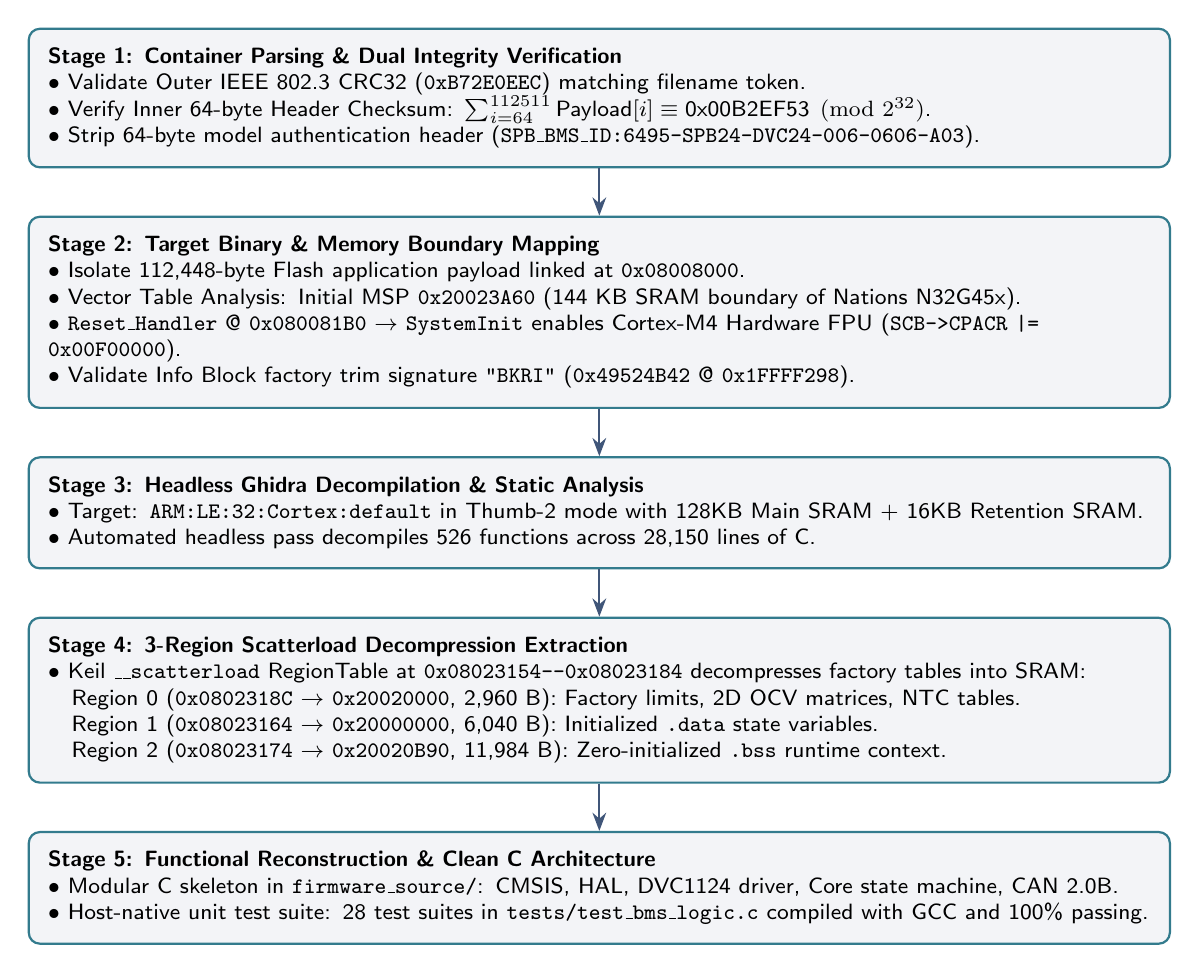
\begin{tikzpicture}[node distance=1.2cm and 1.5cm, auto]
    \node [stagebox, text width=14cm] (s1) {\textbf{Stage 1: Container Parsing \& Dual Integrity Verification}\\
    $\bullet$ Validate Outer IEEE 802.3 CRC32 (\texttt{0xB72E0EEC}) matching filename token.\\
    $\bullet$ Verify Inner 64-byte Header Checksum: $\sum_{i=64}^{112511} \text{Payload}[i] \equiv \text{0x00B2EF53} \pmod{2^{32}}$.\\
    $\bullet$ Strip 64-byte model authentication header (\texttt{SPB\_BMS\_ID:6495-SPB24-DVC24-006-0606-A03}).};

    \node [stagebox, text width=14cm, below=0.6cm of s1] (s2) {\textbf{Stage 2: Target Binary \& Memory Boundary Mapping}\\
    $\bullet$ Isolate 112,448-byte Flash application payload linked at \texttt{0x08008000}.\\
    $\bullet$ Vector Table Analysis: Initial MSP \texttt{0x20023A60} (144 KB SRAM boundary of Nations N32G45x).\\
    $\bullet$ \texttt{Reset\_Handler} @ \texttt{0x080081B0} $\rightarrow$ \texttt{SystemInit} enables Cortex-M4 Hardware FPU (\texttt{SCB->CPACR |= 0x00F00000}).\\
    $\bullet$ Validate Info Block factory trim signature \texttt{"BKRI"} (\texttt{0x49524B42} @ \texttt{0x1FFFF298}).};

    \node [stagebox, text width=14cm, below=0.6cm of s2] (s3) {\textbf{Stage 3: Headless Ghidra Decompilation \& Static Analysis}\\
    $\bullet$ Target: \texttt{ARM:LE:32:Cortex:default} in Thumb-2 mode with 128KB Main SRAM + 16KB Retention SRAM.\\
    $\bullet$ Automated headless pass decompiles 526 functions across 28,150 lines of C.};

    \node [stagebox, text width=14cm, below=0.6cm of s3] (s4) {\textbf{Stage 4: 3-Region Scatterload Decompression Extraction}\\
    $\bullet$ Keil \texttt{\_\_scatterload} RegionTable at \texttt{0x08023154--0x08023184} decompresses factory tables into SRAM:\\
    \quad Region 0 (\texttt{0x0802318C} $\rightarrow$ \texttt{0x20020000}, 2,960 B): Factory limits, 2D OCV matrices, NTC tables.\\
    \quad Region 1 (\texttt{0x08023164} $\rightarrow$ \texttt{0x20000000}, 6,040 B): Initialized \texttt{.data} state variables.\\
    \quad Region 2 (\texttt{0x08023174} $\rightarrow$ \texttt{0x20020B90}, 11,984 B): Zero-initialized \texttt{.bss} runtime context.};

    \node [stagebox, text width=14cm, below=0.6cm of s4] (s5) {\textbf{Stage 5: Functional Reconstruction \& Clean C Architecture}\\
    $\bullet$ Modular C skeleton in \texttt{firmware\_source/}: CMSIS, HAL, DVC1124 driver, Core state machine, CAN 2.0B.\\
    $\bullet$ Host-native unit test suite: 28 test suites in \texttt{tests/test\_bms\_logic.c} compiled with GCC and 100\% passing.};

    \draw [arrow] (s1) -- (s2);
    \draw [arrow] (s2) -- (s3);
    \draw [arrow] (s3) -- (s4);
    \draw [arrow] (s4) -- (s5);
\end{tikzpicture}
\caption{End-to-End BMS Firmware Reverse Engineering \& Extraction Pipeline}
\end{figure}

% ==============================================================================
\section{Microcontroller \& Board Architecture}
% ==============================================================================

\subsection{Hardware Specifications}
\begin{itemize}
    \item \textbf{Microcontroller:} Nations Technologies N32G452 / N32G457 (ARM Cortex-M4F core @ 144 MHz, Single-Precision FPU).
    \item \textbf{Memory Subsystem:} 512 KB embedded Flash memory; 144 KB SRAM partitioned into 128 KB Main SRAM (\texttt{0x20000000--0x2001FFFF}) and 16 KB Battery-Backed Retention SRAM (\texttt{0x20020000--0x20023FFF}).
    \item \textbf{Battery Chemistry \& Topology:} 21 Series, 1 Parallel (21S1P) NCM Lithium-Ion chemistry (nominal cell 3.608 V, stack 75.8 V nominal, 70 Ah nominal pack capacity).
    \item \textbf{Analog Front End (AFE):} Devechip DVC1124-1 precision 24-channel high-voltage battery monitoring IC.
    \item \textbf{Communications:} Isolated CAN 2.0B transceiver (250 kbps), RS-485 / Modbus RTU diagnostic port (9600 baud), and BLE auxiliary serial interface.
\end{itemize}

\subsection{Pinout Map (Board: SPB24-DVC24-006-0606-A03)}
\begin{table}[htbp]
\centering
\caption{Hardware Pin Assignment \& Functional Multiplexing}
\label{tab:pinout}
\begin{tabularx}{\textwidth}{llllX}
\toprule
\textbf{MCU Pin} & \textbf{Type} & \textbf{Signal Name} & \textbf{Polarity} & \textbf{Functional Description} \\
\midrule
\texttt{PA0} & GPIO In & \texttt{ACC\_WAKE} & Active HIGH & Vehicle ignition ACC key input \\
\texttt{PB1} & GPIO In & \texttt{CIN\_DETECT} & Active HIGH & External battery charger insertion detect \\
\texttt{PC2} & GPIO In & \texttt{DIN\_DETECT} & Active HIGH & Vehicle motor controller discharge enable detect \\
\texttt{PA8} & GPIO Out & \texttt{CHG\_EN} & Active HIGH & Main Charging Power MOSFET Gate Driver \\
\texttt{PC9} & GPIO Out & \texttt{DSG\_EN} & Active HIGH & Main Discharging Power MOSFET Gate Driver \\
\texttt{PC4} & GPIO Out & \texttt{PRECHARGE\_EN} & Active HIGH & Inverter capacitive pre-charge current limiting path \\
\texttt{PB6 / PB10} & GPIO Out & \texttt{AFE\_SCL} & Clock & Bit-banged I2C clock to Devechip DVC1124 \\
\texttt{PB7 / PB11} & GPIO I/O & \texttt{AFE\_SDA} & Bi-dir & Bit-banged I2C data line to Devechip DVC1124 \\
\texttt{PA11} & Peripheral & \texttt{CAN\_RX} & Digital & Dedicated CAN1 receive line (250 kbps) \\
\texttt{PA12} & Peripheral & \texttt{CAN\_TX} & Digital & Dedicated CAN1 transmit line (250 kbps) \\
\texttt{PA9} & Peripheral & \texttt{RS485\_TX} & Digital & USART1 transmit line for Modbus / Diagnostic \\
\texttt{PA10} & Peripheral & \texttt{RS485\_RX} & Digital & USART1 receive line for Modbus / Diagnostic \\
\bottomrule
\end{tabularx}
\end{table}

% ==============================================================================
\section{Devechip DVC1124-1 AFE Deep Register Architecture}
% ==============================================================================

\subsection{Physical Layer \& I2C Protocol}
The DVC1124-1 is a 24-channel high-voltage battery monitor IC communicating with the MCU over a dedicated bit-banged I2C interface on \texttt{GPIOB} (\texttt{0x40010C00}) with microsecond timing delays (\texttt{FUN\_080121bc}).
\begin{itemize}
    \item \textbf{7-Bit Slave Address:} \texttt{0x20} (Write: \texttt{0x40}, Read: \texttt{0x41}).
    \item \textbf{Packet Error Checking (PEC / CRC-8):} Every transaction enforces an 8-bit CRC with polynomial $x^8 + x^2 + x + 1$ (\texttt{0x07}):
    \begin{equation}
        \text{CRC8}(X, D) = (X \ll 1) \oplus 0x07 \quad \text{when MSB is set}
    \end{equation}
    \item \textbf{Bus Fault Recovery:} Up to 5 consecutive transaction retries on NACK before declaring communication failure and entering safe shutdown.
\end{itemize}

\subsection{Recovered DVC1124 Register Map}
Table~\ref{tab:dvc1124_regs} documents all registers extracted from decompiled transactions (\texttt{FUN\_080122f0}, \texttt{FUN\_08012760}, \texttt{FUN\_08012720}).

\begin{longtable}{lllcp{7.5cm}}
\caption{Devechip DVC1124-1 Complete Register Map} \label{tab:dvc1124_regs} \\
\toprule
\textbf{Address} & \textbf{Register Name} & \textbf{Access} & \textbf{Bytes} & \textbf{Functional Description} \\
\midrule
\endfirsthead
\multicolumn{5}{c}%
{{\bfseries \tablename\ \thetable{} -- continued from previous page}} \\
\toprule
\textbf{Address} & \textbf{Register Name} & \textbf{Access} & \textbf{Bytes} & \textbf{Functional Description} \\
\midrule
\endhead
\midrule
\multicolumn{5}{r}{{Continued on next page}} \\
\bottomrule
\endfoot
\bottomrule
\endlastfoot
\texttt{0x00} & \texttt{DVC\_REG\_SYS\_CTRL} & R/W & 1 & System Control (Soft Reset, Sleep entry, Wakeup trigger) \\
\texttt{0x01} & \texttt{DVC\_REG\_CELL\_MODE} & R/W & 1 & Series Cell Count Mode (\texttt{0x0D} = 21S, \texttt{0x0E} = 22S, \texttt{0x0F} = 24S) \\
\texttt{0x02} & \texttt{DVC\_REG\_CURRENT} & Read & 2 & Signed 16-bit Pack Current ADC reading (5 mA/LSB) \\
\texttt{0x06} & \texttt{DVC\_REG\_ADC\_CTRL} & R/W & 1 & ADC Channel Sequencing \& Internal Oscillator Enable \\
\texttt{0x07} & \texttt{DVC\_REG\_ADC\_CONFIG} & R/W & 2 & ADC Sample Rate, Decimation Rate \& Digital Averaging Filter \\
\texttt{0x0B} & \texttt{DVC\_REG\_CELL\_STATUS} & Read & 2 & Hardware Alert Flags \& Cell Voltage Measurement Status \\
\texttt{0x0F} & \texttt{DVC\_REG\_NTC\_BASE} & Read & 14 & NTC Thermistor ADC Channels (up to 6 thermistor sensors) \\
\texttt{0x1D} & \texttt{DVC\_REG\_CELL\_VOLTAGES} & Read & 42 & 21-Cell Voltage ADC readings ($21 \times 2$ bytes, 0.1 mV/LSB) \\
\texttt{0x4F} & \texttt{DVC\_REG\_PACK\_VOLTAGE} & Read & 2 & Total High-Voltage Stack Voltage ADC reading \\
\texttt{0x51} & \texttt{DVC\_REG\_MEAS\_CTRL} & R/W & 1 & Measurement Trigger (Bit 7 = Trigger Scan, Bits [3:2] = Mode) \\
\texttt{0x52} & \texttt{DVC\_REG\_BURST\_CELLS} & R/W & 40/3 & Burst cell read (\texttt{0x28} B) / Diagnostic burst write (3 B) \\
\texttt{0x56} & \texttt{DVC\_REG\_BALANCING\_CTRL} & Write & 36 & Passive Balancing Control Matrix \& Hardware Trip Thresholds \\
\texttt{0x5A} & \texttt{DVC\_REG\_FAULT\_STATUS} & R/W & 1 & Hardware Fault Status Register (Cleared by writing \texttt{0xFE}) \\
\texttt{0x5E} & \texttt{DVC\_REG\_OVP\_THRESH} & R/W & 1 & Hardware Over-Voltage Cutoff Threshold \\
\texttt{0x5F} & \texttt{DVC\_REG\_OVP\_DELAY} & R/W & 1 & Hardware Over-Voltage Filter Debounce Delay \\
\texttt{0x60} & \texttt{DVC\_REG\_UVP\_THRESH} & R/W & 1 & Hardware Under-Voltage Cutoff Threshold \\
\texttt{0x61} & \texttt{DVC\_REG\_UVP\_DELAY} & R/W & 1 & Hardware Under-Voltage Filter Debounce Delay \\
\texttt{0x62} & \texttt{DVC\_REG\_TEMP\_CONFIG} & R/W & 1 & NTC Sensor Channel Configuration \& Multiplexer Enable \\
\texttt{0x63} & \texttt{DVC\_REG\_CHG\_OCP} & R/W & 1 & Hardware Charge Over-Current Protection Threshold \\
\texttt{0x67} & \texttt{DVC\_REG\_DSG\_OCP1} & R/W & 1 & Hardware Discharge Over-Current Level 1 Threshold \\
\texttt{0x68} & \texttt{DVC\_REG\_DSG\_OCP2} & R/W & 1 & Hardware Discharge Short-Circuit Level 2 Threshold \\
\texttt{0x69} & \texttt{DVC\_REG\_OCP\_DELAY} & R/W & 1 & Over-Current Protection Trip Debounce Filter Delay \\
\texttt{0x6E} & \texttt{DVC\_REG\_AFE\_CONFIG} & R/W & 1 & AFE Core Analog Configuration (\texttt{0xCD} normal / \texttt{0x8D}) \\
\texttt{0x7E} & \texttt{DVC\_REG\_CHIP\_ID\_VREF} & Read & 1 & Chip Silicon ID \& Internal VREF Trim Calibration \\
\texttt{0x8E} & \texttt{DVC\_REG\_RESET\_DIAG} & R/W & 1 & AFE Soft Reset \& Hardware Self-Diagnostic Control (\texttt{0x80}) \\
\end{longtable}

\subsection{Sensor Measurement \& Mathematical Conversion Formulas}
Decompiled arithmetic routines and Flash literal pools define the exact sensor conversion scaling:
\begin{enumerate}
    \item \textbf{Cell Voltage Conversion (\texttt{FUN\_0800d218} @ \texttt{0x0800D218}):}
    Gain \texttt{DAT\_0800d3bc} $= 0.0001\text{f}$ ($0.1\text{ mV/count}$), Offset \texttt{DAT\_0800d3c0} $= 0.0005\text{f}$ ($0.5\text{ mV}$):
    \begin{equation}
        V_{\text{cell}} (\text{mV}) = (\text{Raw ADC Counts} \times 0.1) + 0.5
    \end{equation}
    \item \textbf{Pack Current Conversion (\texttt{FUN\_0800d48c} @ \texttt{0x0800D48C}):}
    Shunt scaling factor \texttt{DAT\_0800d52c} $= 0.005\text{f}$ ($5\text{ mA/count}$):
    \begin{equation}
        I_{\text{pack}} (\text{mA}) = -(\text{Raw ADC Counts} - I_{\text{zero\_offset}}) \times 5.0
    \end{equation}
    \textit{(Negative values denote discharge current into the powertrain; positive values denote charge current from EVSE or regen).}
    \item \textbf{NTC Temperature Conversion (\texttt{FUN\_0800cfc0} @ \texttt{0x0800CFC0}):}
    Evaluates the ADC ratio against VREF trim (\texttt{0x7E}), indexes a 160-point calibration curve, and applies a $-40^\circ\text{C}$ offset:
    \begin{equation}
        T (^\circ\text{C}) = \text{LookupIndex} - 40
    \end{equation}
    \item \textbf{Per-Cell Voltage Gain Multipliers (\texttt{FUN\_08016000} @ \texttt{0x08016000}):}
    Reads 21 discrete calibration words from EEPROM \texttt{0x0060}, divides each by constant \texttt{DAT\_08016140}, validates safety bounds (defaulting to \texttt{1.0f} if uncalibrated), and multiplies each cell reading individually.
\end{enumerate}

\subsection{Multi-AFE Chip Family Support \& 3-Phase Interleaved Balancing}
\begin{itemize}
    \item \textbf{Dynamic Chip Family Dispatch (\texttt{FUN\_08008af4} \& \texttt{FUN\_08013a04}):}
    The firmware branches dynamically based on the configured chip model ID (\texttt{*DAT\_08009bd4}):
    \texttt{0x0464} ($1124_{10}$) for Devechip DVC1124 (24S), \texttt{0x045D} ($1117_{10}$) for DVC1117 (17S), and \texttt{0x045A} ($1114_{10}$) for DVC1114 (14S).
    \item \textbf{3-Phase Interleaved Passive Balancing (\texttt{FUN\_08008af4}):}
    Passive bleed resistors generate significant heat. To prevent localized PCB hot-spots and sense-wire voltage sag, the firmware splits the 21-cell balancing mask into \textbf{3 non-adjacent interleaved phases} cycling every 20--50 seconds:
    \begin{equation}
        \text{Phase 0: Cells } \{1, 4, 7, 10, 13, 16, 19\} \quad (\text{Mask } \texttt{0x049249})
    \end{equation}
    \begin{equation}
        \text{Phase 1: Cells } \{2, 5, 8, 11, 14, 17, 20\} \quad (\text{Mask } \texttt{0x092492})
    \end{equation}
    \begin{equation}
        \text{Phase 2: Cells } \{3, 6, 9, 12, 15, 18, 21\} \quad (\text{Mask } \texttt{0x124924})
    \end{equation}
    This ensures that two physically adjacent cells never bleed simultaneously.
\end{itemize}

% ==============================================================================
\section{Core BMS State Machine \& Protection Engine}
% ==============================================================================

\subsection{Calibrated Safety Thresholds}
Extracted from Scatterload Decompression Table \texttt{0x08023184} into Retention SRAM \texttt{0x20020000}:
\begin{table}[htbp]
\centering
\caption{Calibrated System Safety Thresholds \& Trigger Delays}
\label{tab:safety_thresholds}
\begin{tabularx}{\textwidth}{lrrrl}
\toprule
\textbf{Protection Parameter} & \textbf{Trip Threshold} & \textbf{Release Threshold} & \textbf{Trip Delay} & \textbf{Firmware Action} \\
\midrule
\textbf{Cell Over-Voltage (OVP)} & $4,185\text{ mV}$ & $4,100\text{ mV}$ & $100\text{ ms}$ & Open CHG MOSFET (\texttt{PA8 = LOW}) \\
\textbf{Cell Balancing Start} & $4,120\text{ mV}$ & $\Delta V < 20\text{ mV}$ & Continuous & Engage 3-phase bleed via \texttt{Reg 0x56} \\
\textbf{Nominal Cell Voltage} & $3,608\text{ mV}$ & --- & --- & Baseline 50\% SOC nominal voltage \\
\textbf{Under-Voltage Warning (UVW)} & $2,831\text{ mV}$ & $3,000\text{ mV}$ & $500\text{ ms}$ & Broadcast dashboard derating alert on CAN \\
\textbf{Under-Voltage Cutoff (UVC)} & $2,621\text{ mV}$ & CIN active & $100\text{ ms}$ & Open DSG MOSFET (\texttt{PC9 = LOW}) \\
\textbf{Charge Over-Temperature (OTC)} & $+55^\circ\text{C}$ & $+50^\circ\text{C}$ & $1000\text{ ms}$ & Inhibit charging, open CHG MOSFET \\
\textbf{Discharge Over-Temp (OTD)} & $+65^\circ\text{C}$ & $+60^\circ\text{C}$ & $1000\text{ ms}$ & Open DSG MOSFET, isolate powertrain \\
\textbf{MOSFET Over-Temperature} & $+85^\circ\text{C}$ & $+75^\circ\text{C}$ & $500\text{ ms}$ & Emergency open of both CHG \& DSG MOSFETs \\
\textbf{Auxiliary Path Current Limit} & $2.0\text{ A}$ & DIN active & $200\text{ ms}$ & Prevent quiescent key ACC battery drain \\
\bottomrule
\end{tabularx}
\end{table}

\subsection{MOSFET Interlocking \& Pre-Charge Sequencing}
\begin{itemize}
    \item \textbf{Discharge Interlock:} Discharging is strictly permitted when:
    \begin{equation}
        (\texttt{PA0} == \text{HIGH}) \;\land\; (\texttt{PC2} == \text{HIGH}) \;\land\; (\text{faults.all} == 0)
    \end{equation}
    \item \textbf{Pre-Charge Sequence (\texttt{FUN\_0801647c}):} Closing a discharge contactor into an uncharged motor controller capacitor causes destructive current spikes. The firmware asserts \texttt{PC4} (\texttt{PRECHARGE\_EN}) through a current-limiting resistor. If the capacitor bus voltage fails to rise to pack potential within 10 ticks (1.0 s), it trips pre-charge fault state \texttt{0x11}, shuts all MOSFETs, and logs Black-Box Fault \texttt{0xBE}.
    \item \textbf{Body-Diode Thermal Bypass (\texttt{FUN\_0801f580}):} If the Charge MOSFET is turned OFF (e.g. OVP) while strong discharge current flows through its parasitic internal body diode (forward drop $\approx 0.7\text{ V}$, generating tens of watts of heat), the firmware actively commands the MOSFET gate \textbf{ON} while current persists to bypass the diode via the low-$R_{DS(on)}$ channel, returning it \textbf{OFF} once current subsides.
\end{itemize}

% ==============================================================================
\section{Dynamic State of Health (SOH) \& Capacity Learning}
% ==============================================================================

\subsection{Cycle Degradation Model (\texttt{FUN\_080207fc})}
In the 1-second supervisor task, battery SOH is calculated using a linear cycle decay model:
\begin{equation}
    \text{SOH}_{\text{cycle}} = \max\left(0.0,\; 100.0 - (\text{cycle\_count} \times 0.02)\right)
\end{equation}
\begin{itemize}
    \item Degradation Slope: $0.02\% / \text{cycle}$ (initialized at Flash \texttt{0x08015310}).
    \item $0\text{ Cycles} \rightarrow 100\%\text{ SOH}$ ($70,000\text{ mAh}$ usable).
    \item $1,000\text{ Cycles} \rightarrow 80\%\text{ SOH}$ ($56,000\text{ mAh}$ usable --- EV pack retirement threshold).
\end{itemize}

\subsection{2D Chemical Lookup Matrices}
Decompressed from Scatterload Table \texttt{0x08023184} into Retention SRAM:

\subsubsection{1. Chemical OCV Baseline at 25$^\circ$C (21S 70Ah NCM)}
The open-circuit voltage curve spans 21 points ($100\%$ down to $0\%$ in $5\%$ increments):
\texttt{100\%}: $4,185\text{ mV}$ | \texttt{95\%}: $4,100\text{ mV}$ | \texttt{90\%}: $4,040\text{ mV}$ | \texttt{85\%}: $3,980\text{ mV}$ | \texttt{80\%}: $3,920\text{ mV}$ | \texttt{75\%}: $3,870\text{ mV}$ | \texttt{70\%}: $3,820\text{ mV}$ | \texttt{65\%}: $3,770\text{ mV}$ | \texttt{60\%}: $3,720\text{ mV}$ | \texttt{55\%}: $3,670\text{ mV}$ | \texttt{50\%}: $3,608\text{ mV}$ (Nominal) | \texttt{45\%}: $3,560\text{ mV}$ | \texttt{40\%}: $3,510\text{ mV}$ | \texttt{35\%}: $3,460\text{ mV}$ | \texttt{30\%}: $3,400\text{ mV}$ | \texttt{25\%}: $3,340\text{ mV}$ | \texttt{20\%}: $3,260\text{ mV}$ | \texttt{15\%}: $3,160\text{ mV}$ | \texttt{10\%}: $3,020\text{ mV}$ | \texttt{5\%}: $2,831\text{ mV}$ (Warning) | \texttt{0\%}: $2,621\text{ mV}$ (Cutoff).

\subsubsection{2. Table 1: Chemical Capacity Availability / Discharge C-Rate Matrix ($21 \times 12$)}
\begin{itemize}
    \item \textbf{SRAM Address:} \texttt{0x20020572} (evaluated in \texttt{FUN\_08010654}).
    \item \textbf{Purpose:} 2D Dynamic Discharge C-Rate Limiter mapping SOC and temperature to maximum continuous discharge current for the motor controller/VCU.
    \item \textbf{Dimensions:} 21 Rows ($100\%$ to $0\%$ in $5\%$ steps) $\times$ 12 Temperature Columns ($<-20, -10, 0, 10, 15, 25, 40, 45, 50, 55, 60, \ge 60^\circ\text{C}$).
    \item \textbf{Mathematical Formula (\texttt{FUN\_08010654}):}
    \begin{equation}
        \text{Discharge C-Rate} = \text{Matrix}[row][col] \times 0.1 \quad (0.0\text{ C to }2.0\text{ C})
    \end{equation}
    \begin{equation}
        I_{\text{max\_dsg}} (\text{A}) = \min\!\left(\text{Discharge C-Rate} \times \frac{\text{Pack\_Capacity\_mAh}}{1000.0},\; \text{DSG\_OCP\_Limit\_A} - 1.0\right)
    \end{equation}
    \item \textbf{70 Ah Pack Examples:}
    \begin{itemize}
        \item $85\text{--}100\%\text{ SOC}, 25\text{--}40^\circ\text{C}$: Entry \texttt{20} $\rightarrow 2.0\text{ C} \times 70\text{ Ah} = 140\text{ A}$ (clamped to OCP limit).
        \item $50\%\text{ SOC}, 15\text{--}25^\circ\text{C}$: Entry \texttt{15} $\rightarrow 1.5\text{ C} \times 70\text{ Ah} = 105\text{ A}$ (clamped to OCP limit).
        \item $30\%\text{ SOC}, 15\text{--}25^\circ\text{C}$: Entry \texttt{10} $\rightarrow 1.0\text{ C} \times 70\text{ Ah} = 70\text{ A}$.
        \item $10\%\text{ SOC}, 25\text{--}40^\circ\text{C}$: Entry \texttt{5} $\rightarrow 0.5\text{ C} \times 70\text{ Ah} = 35\text{ A}$ (limp-home mode to prevent UVP sag).
        \item $40\%\text{ SOC}, 0\text{--}10^\circ\text{C}$: Entry \texttt{4} $\rightarrow 0.4\text{ C} \times 70\text{ Ah} = 28\text{ A}$ (cold internal impedance derating).
        \item Extreme Cold ($<-20^\circ\text{C}$) or Over-Temp ($\ge 60^\circ\text{C}$): Entry \texttt{0} $\rightarrow 0.0\text{ C} = 0\text{ A}$ (discharge forbidden).
    \end{itemize}
    \item \textbf{CAN Broadcast \& Overload Throttling (\texttt{FUN\_0801b55c}):} Transmitted in Byte \texttt{D6} of CAN ID \texttt{0x141F1001}. If measured discharge current exceeds $I_{\text{max\_dsg}} + 3.0\text{ A}$ for $>20$ ticks, the BMS dynamically steps the advertised limit down.
\end{itemize}

\subsubsection{3. Table 2: Dynamic Charge Current C-Rate Matrix ($21 \times 13$)}
\begin{itemize}
    \item \textbf{SRAM Address:} \texttt{0x20020720} (evaluated in \texttt{FUN\_080103c8}).
    \item \textbf{Purpose:} 2D Dynamic Charge Current C-Rate Limiter / CC-CV Taper Map commanding the external charger via CAN ID \texttt{0x1806E5F4}.
    \item \textbf{Dimensions:} 21 Rows ($100\%$ to $0\%$) $\times$ 13 Temperature Columns ($<0, 5, 10, 15, 20, 25, 30, 35, 40, 44, 46, 51, \ge 51^\circ\text{C}$).
    \item \textbf{Cold Override:} If minimum cell temperature $<0^\circ\text{C}$, \texttt{FUN\_080103c8} forces Column 0 ($0\text{ A}$) to prevent lithium plating.
    \item \textbf{Mathematical Formula (\texttt{FUN\_080103c8}):}
    \begin{equation}
        \text{Charge C-Rate} = \text{Matrix}[row][col] \times 0.01 \quad (0.00\text{ C to }0.50\text{ C})
    \end{equation}
    \begin{equation}
        I_{\text{max\_chg}} (\text{A}) = \min\!\left(\text{Charge C-Rate} \times \frac{\text{Pack\_Capacity\_mAh}}{1000.0},\; \text{CHG\_OCP\_Limit\_A} - 1.0\right)
    \end{equation}
    \item \textbf{70 Ah Pack Examples:}
    \begin{itemize}
        \item $0\text{--}60\%\text{ SOC}, 25\text{--}39^\circ\text{C}$: Entry \texttt{50} $\rightarrow 0.50\text{ C} \times 70\text{ Ah} = 35.0\text{ A}$ (matches \texttt{0x0042} OCP Chg).
        \item $50\%\text{ SOC}, 15\text{--}19^\circ\text{C}$: Entry \texttt{40} $\rightarrow 0.40\text{ C} \times 70\text{ Ah} = 28.0\text{ A}$.
        \item $80\text{--}95\%\text{ SOC}, 25\text{--}34^\circ\text{C}$: Entry \texttt{30} $\rightarrow 0.30\text{ C} \times 70\text{ Ah} = 21.0\text{ A}$ (CV taper region).
        \item $95\%\text{ SOC}, 0\text{--}9^\circ\text{C}$: Entry \texttt{10} $\rightarrow 0.10\text{ C} \times 70\text{ Ah} = 7.0\text{ A}$ (cold trickle charge).
        \item $100\%\text{ SOC}$ (any temp), $<0^\circ\text{C}$, or $\ge 51^\circ\text{C}$: Entry \texttt{0} $\rightarrow 0.00\text{ C} = 0.0\text{ A}$ (charging inhibited).
    \end{itemize}
\end{itemize}

\subsection{Hybrid SOC Estimator Architecture}
Neither voltage nor current alone provides reliable SOC: voltage suffers from internal resistance ($I \cdot R$) and polarization sag under load, while Coulomb counting drifts over days due to shunt offsets. The firmware fuses both in a multi-stage hybrid engine.

\begin{figure}[htbp]
\centering
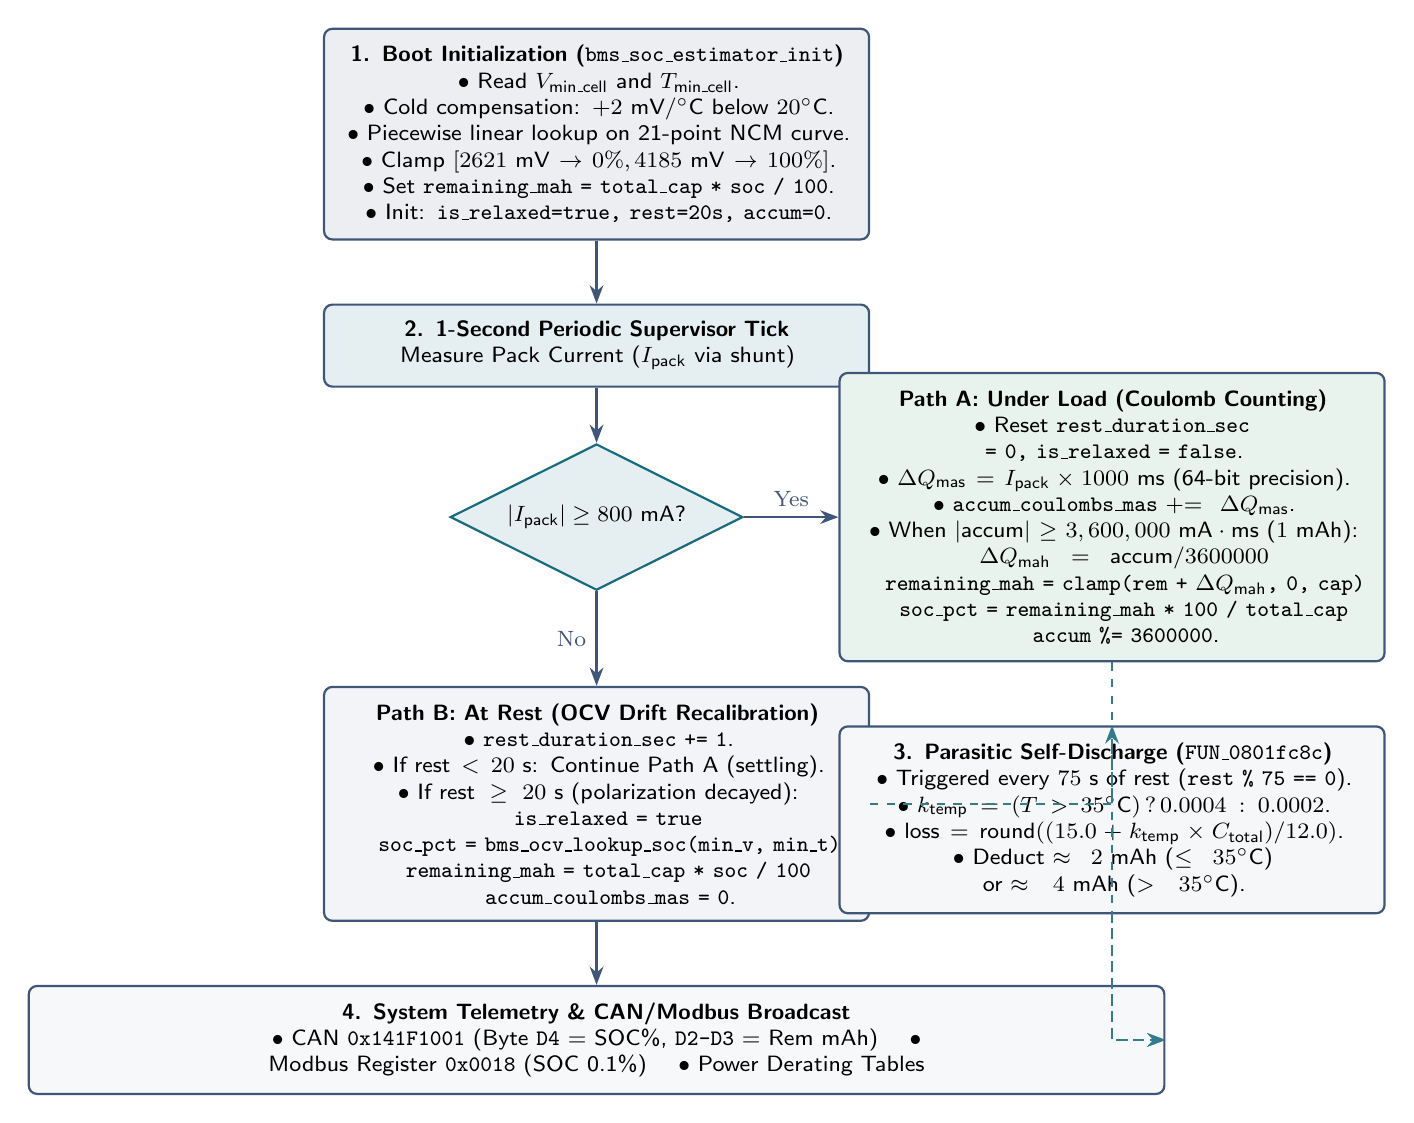
\begin{tikzpicture}[node distance=1.0cm and 1.2cm, auto]
    % Boot Box
    \node [box, text width=6.5cm, fill=NavyBlue!8] (boot) {
        \textbf{1. Boot Initialization (\texttt{bms\_soc\_estimator\_init})}\\
        $\bullet$ Read $V_{\text{min\_cell}}$ and $T_{\text{min\_cell}}$.\\
        $\bullet$ Cold compensation: $+2\text{ mV}/^\circ\text{C}$ below $20^\circ\text{C}$.\\
        $\bullet$ Piecewise linear lookup on 21-point NCM curve.\\
        $\bullet$ Clamp $[2621\text{ mV} \rightarrow 0\%, 4185\text{ mV} \rightarrow 100\%]$.\\
        $\bullet$ Set \texttt{remaining\_mah = total\_cap * soc / 100}.\\
        $\bullet$ Init: \texttt{is\_relaxed=true, rest=20s, accum=0}.
    };

    % 1s Tick
    \node [box, below=0.8cm of boot, text width=6.5cm, fill=DarkTeal!10] (tick) {
        \textbf{2. 1-Second Periodic Supervisor Tick}\\
        Measure Pack Current ($I_{\text{pack}}$ via shunt)
    };

    % Decision
    \node [decision, below=0.7cm of tick] (dec) {$|I_{\text{pack}}| \ge 800\text{ mA}$?};

    % Path A (Load)
    \node [box, right=1.2cm of dec, text width=6.5cm, fill=AccentGreen!10] (load) {
        \textbf{Path A: Under Load (Coulomb Counting)}\\
        $\bullet$ Reset \texttt{rest\_duration\_sec = 0, is\_relaxed = false}.\\
        $\bullet$ $\Delta Q_{\text{mas}} = I_{\text{pack}} \times 1000\text{ ms}$ (64-bit precision).\\
        $\bullet$ \texttt{accum\_coulombs\_mas} $\mathrel{+}= \Delta Q_{\text{mas}}$.\\
        $\bullet$ When $|\text{accum}| \ge 3,600,000\text{ mA}\cdot\text{ms}$ ($1\text{ mAh}$):\\
        \quad $\Delta Q_{\text{mah}} = \text{accum} / 3600000$\\
        \quad \texttt{remaining\_mah = clamp(rem + }$\Delta Q_{\text{mah}}$\texttt{, 0, cap)}\\
        \quad \texttt{soc\_pct = remaining\_mah * 100 / total\_cap}\\
        \quad \texttt{accum \%= 3600000}.
    };

    % Path B (Rest)
    \node [box, below=1.2cm of dec, text width=6.5cm, fill=NavyBlue!5] (rest) {
        \textbf{Path B: At Rest (OCV Drift Recalibration)}\\
        $\bullet$ \texttt{rest\_duration\_sec += 1}.\\
        $\bullet$ If $\text{rest} < 20\text{ s}$: Continue Path A (settling).\\
        $\bullet$ If $\text{rest} \ge 20\text{ s}$ (polarization decayed):\\
        \quad \texttt{is\_relaxed = true}\\
        \quad \texttt{soc\_pct = bms\_ocv\_lookup\_soc(min\_v, min\_t)}\\
        \quad \texttt{remaining\_mah = total\_cap * soc / 100}\\
        \quad \texttt{accum\_coulombs\_mas = 0}.
    };

    % Self Discharge
    \node [box, below=0.8cm of load, text width=6.5cm, fill=BorderGray!20] (selfdsg) {
        \textbf{3. Parasitic Self-Discharge (\texttt{FUN\_0801fc8c})}\\
        $\bullet$ Triggered every $75\text{ s}$ of rest (\texttt{rest \% 75 == 0}).\\
        $\bullet$ $k_{\text{temp}} = (T > 35^\circ\text{C})\,?\,0.0004 : 0.0002$.\\
        $\bullet$ $\text{loss} = \text{round}((15.0 + k_{\text{temp}} \times C_{\text{total}}) / 12.0)$.\\
        $\bullet$ Deduct $\approx 2\text{ mAh}$ ($\le 35^\circ\text{C}$) or $\approx 4\text{ mAh}$ ($>35^\circ\text{C}$).
    };

    % Output
    \node [box, below=0.8cm of rest, text width=14cm, fill=LightGray] (out) {
        \textbf{4. System Telemetry \& CAN/Modbus Broadcast}\\
        $\bullet$ CAN \texttt{0x141F1001} (Byte \texttt{D4} = SOC\%, \texttt{D2-D3} = Rem mAh) \quad
        $\bullet$ Modbus Register \texttt{0x0018} (SOC 0.1\%) \quad
        $\bullet$ Power Derating Tables
    };

    \draw [arrow] (boot) -- (tick);
    \draw [arrow] (tick) -- (dec);
    \draw [arrow] (dec) -- node[above]{\footnotesize Yes} (load);
    \draw [arrow] (dec) -- node[left]{\footnotesize No} (rest);
    \draw [dashedarrow] (load) |- (out);
    \draw [arrow] (rest) -- (out);
    \draw [dashedarrow] (rest) -| (selfdsg);
    \draw [dashedarrow] (selfdsg) |- (out);
\end{tikzpicture}
\caption{Hybrid SOC Estimator Multi-Stage Architecture}
\label{fig:soc_estimator}
\end{figure}

% ==============================================================================
\section{CAN 2.0B Communication Matrix (250 kbps)}
% ==============================================================================

\subsection{29-Bit Extended Identifier Layout}
Disassembly of Thumb-2 instructions in ID packer \texttt{FUN\_0801ef94} (\texttt{0x0801EF94}) and unpacker \texttt{FUN\_0800daf4} (\texttt{0x0800DAF4}) confirms the 29-bit CAN ID structure:
\begin{equation}
    \text{CAN\_ID}_{29} = (\text{SID}_{4:0} \ll 24) \;\mid\; (\text{DID}_{4:0} \ll 16) \;\mid\; (\text{CMD}_{7:0} \ll 8) \;\mid\; \text{Index}_{7:0}
\end{equation}
\begin{itemize}
    \item \textbf{Bits [28:24] (SID):} Source Node ID (Master BMS = \texttt{0x14}, Slave BMS = \texttt{0x1D}, VCU = \texttt{0x01}).
    \item \textbf{Bits [23:21]:} Reserved (\texttt{0b000}).
    \item \textbf{Bits [20:16] (DID):} Destination Node ID (Target node or Broadcast = \texttt{0x1F}).
    \item \textbf{Bits [15:8] (CMD):} Primary Command Code.
    \item \textbf{Bits [7:0] (Index):} Sub-Command / Parameter Index.
    \item \textbf{Endianness:} All multi-byte data fields are strictly \textbf{Little-Endian} (LSB first).
\end{itemize}

\subsection{Periodic Broadcast Schedule \& Command Matrix}
\begin{longtable}{lllcp{7.5cm}}
\caption{CAN 2.0B Frame Matrix (250 kbps)} \label{tab:can_matrix} \\
\toprule
\textbf{Frame Description} & \textbf{Identifier / CMD} & \textbf{Period} & \textbf{DLC} & \textbf{Payload Byte Layout (Little-Endian)} \\
\midrule
\endfirsthead
\multicolumn{5}{c}%
{{\bfseries \tablename\ \thetable{} -- continued from previous page}} \\
\toprule
\textbf{Frame Description} & \textbf{Identifier / CMD} & \textbf{Period} & \textbf{DLC} & \textbf{Payload Byte Layout (Little-Endian)} \\
\midrule
\endhead
\midrule
\multicolumn{5}{r}{{Continued on next page}} \\
\bottomrule
\endfoot
\bottomrule
\endlastfoot
\textbf{Broadcast: Fault Status} & \texttt{0x141F0E<ERR>} & 1000 ms & 8 & \texttt{Index=ERR}; \texttt{D0..D7}: 64-bit protection fault bitmask \\
\textbf{Broadcast: Capacity \& SOC} & \texttt{0x141F1001} & 100 ms & 7 & \texttt{D0-D1}: FCC ($10\text{ mAh}$), \texttt{D2-D3}: Rem ($10\text{ mAh}$), \texttt{D4}: SOC\%, \texttt{D5}: SOH\%, \texttt{D6}: Max DSG Current (A) \\
\textbf{Broadcast: Telemetry I/V/T} & \texttt{0x141F1002} & 100 ms & 8 & \texttt{D0}: State (0=Idle, 1=Chg, 2=Dsg), \texttt{D1-D2}: Current ($0.01\text{ A}$), \texttt{D3-D5}: 24-bit Pack V ($1\text{ mV}$), \texttt{D6-D7}: Min/Max T ($+40^\circ\text{C}$) \\
\textbf{Broadcast: Switch / MOS} & \texttt{0x141F1040} & 1000 ms & 7 & \texttt{D0}: DsgSwitch, \texttt{D1}: Addr, \texttt{D2}: Charger, \texttt{D3}: Load, \texttt{D4}: DSG MOS, \texttt{D5}: CHG MOS, \texttt{D6}: Key ACC \\
\textbf{Broadcast: Parallel Status} & \texttt{0x141F1101} & 100 ms & 5 & \texttt{D0}: ParallelFlag, \texttt{D1}: ActiveBat (1/2), \texttt{D2}: Charger, \texttt{D3}: SwitchState, \texttt{D4}: BatCount \\
\textbf{Broadcast: Pack Rating} & \texttt{0x141F1201} & 1000 ms & 8 & \texttt{D0}: 21S, \texttt{D1}: 1P, \texttt{D2-D3}: 7000 ($10\text{ mAh}$), \texttt{D4}: MaxChgI ($0.4\text{ A}$), \texttt{D5}: MaxDsgI ($1\text{ A}$), \texttt{D6-D7}: Cycles \\
\textbf{OBC Charger Control} & \texttt{0x1806E5F4} & 1000 ms & 8 & \texttt{D0-D1}: Target V ($0.1\text{ V}$), \texttt{D2-D3}: Max I ($0.1\text{ A}$), \texttt{D4}: Stop/Allow flag (SAE J1939 OBC) \\
\textbf{P2P: Cell Voltages 1--24} & \texttt{CMD=0x41, IDX=03..08} & On Query & 8 & 4 cells/frame, 16-bit Little-Endian mV per cell (\texttt{0x0801BE1A}) \\
\textbf{P2P: Cell Balancing Mask} & \texttt{CMD=0x42, IDX=10..12} & On Query & 8 & 8 cells/frame (\texttt{1} = balancing active, \texttt{0} = idle) \\
\textbf{P2P: Long Packet Multi-Frame} & \texttt{CMD=0x04, IDX=1..N} & On Query & 8 & \texttt{[OrigCMD, SubCMD, LenLo, LenHi, Data..., CRC16\_Lo, CRC16\_Hi]} \\
\textbf{P2P: OTA Boot Trigger} & \texttt{CMD=0x1A, IDX=0x00} & Async & 6 & Payload \texttt{"UPDATE"}: Writes \texttt{0x28A} Flash flag \& soft resets MCU \\
\textbf{Internal Parallel Bus} & \texttt{0x141DF001} & 100 ms & 8 & Inter-pack dual-battery parallel arbitration (\texttt{FUN\_0801ca08}) \\
\end{longtable}

% ==============================================================================
\section{RS-485 / Modbus RTU \& PC Diagnostic Protocol Engine}
% ==============================================================================

\subsection{Unified 7-Port Serial Driver}
The firmware implements an abstracted serial driver supporting all 7 UART controllers of the N32G45x (\texttt{USART1..3}, \texttt{UART4..7}) with dynamic direction switching for half-duplex RS-485 DE/RE pins in \texttt{FUN\_08016420}. Default framing: 9600 baud, 8 data bits, no parity, 1 stop bit (8N1).

\subsection{Modbus Register Map}
CRC-16 polynomial: standard Modbus \texttt{0xA001} (seed \texttt{0xFFFF}, LSB first). Supported Function Codes: \texttt{0x03} (Read Holding), \texttt{0x04} (Read Input), \texttt{0x06} (Write Single), and \texttt{0x10} (Write Multiple).

\begin{table}[htbp]
\centering
\caption{Modbus RTU Register Allocation Map}
\label{tab:modbus_regs}
\begin{tabularx}{\textwidth}{lllrX}
\toprule
\textbf{Register} & \textbf{Type} & \textbf{Units} & \textbf{Scale} & \textbf{Parameter Description} \\
\midrule
\texttt{0x0001--0x0015} & \texttt{uint16\_t} & mV & $1$ & Individual Cell Voltages 1 through 21 \\
\texttt{0x0016} & \texttt{uint16\_t} & mV & $10$ & Total Battery Pack Voltage ($7660 \rightarrow 76.60\text{ V}$) \\
\texttt{0x0017} & \texttt{int16\_t} & mA & $10$ & Battery Current (signed: $+$ chg, $-$ dsg) \\
\texttt{0x0018} & \texttt{uint16\_t} & \% & $0.1$ & State of Charge ($0\dots 1000 \rightarrow 0.0\dots 100.0\%$) \\
\texttt{0x0019} & \texttt{uint16\_t} & \% & $0.1$ & State of Health ($0\dots 1000 \rightarrow 0.0\dots 100.0\%$) \\
\texttt{0x001A} & \texttt{uint16\_t} & Ah & $0.1$ & Remaining Usable Capacity ($350 \rightarrow 35.0\text{ Ah}$) \\
\texttt{0x001B} & \texttt{uint16\_t} & Ah & $0.1$ & Full Learned Capacity ($700 \rightarrow 70.0\text{ Ah}$) \\
\texttt{0x001C} & \texttt{uint16\_t} & Cycles & $1$ & Lifetime Full Equivalent Discharge Cycles \\
\texttt{0x001D} & \texttt{uint16\_t} & mV & $1$ & Maximum Cell Voltage ($\max V_{\text{cell}}$) \\
\texttt{0x001E} & \texttt{uint16\_t} & mV & $1$ & Minimum Cell Voltage ($\min V_{\text{cell}}$) \\
\texttt{0x001F} & \texttt{uint16\_t} & mV & $1$ & Cell Voltage Imbalance Delta ($\Delta V = \max - \min$) \\
\texttt{0x0020--0x0023} & \texttt{int16\_t} & $^\circ\text{C}$ & $0.1$ & Cell Thermistor Temperatures NTC 1 through 4 \\
\texttt{0x0024} & \texttt{int16\_t} & $^\circ\text{C}$ & $0.1$ & Power MOSFET Stage Temperature \\
\texttt{0x0025} & \texttt{int16\_t} & $^\circ\text{C}$ & $0.1$ & Ambient Enclosure Temperature \\
\texttt{0x0030} & \texttt{uint16\_t} & Enum & $1$ & State ($0$: Init, $1$: Standby, $2$: Chg, $3$: Dsg, $4$: Fault) \\
\texttt{0x0031} & \texttt{uint16\_t} & Bitfield & --- & Active Protection / Fault Bitmask \\
\texttt{0x0032} & \texttt{uint16\_t} & Bitfield & --- & MOSFET State (Bit 0: CHG MOS, Bit 1: DSG MOS) \\
\texttt{0x0040} & \texttt{uint16\_t} & mV & $1$ & Over-Voltage Protection Threshold ($4,185\text{ mV}$) \\
\texttt{0x0041} & \texttt{uint16\_t} & mV & $1$ & Under-Voltage Protection Threshold ($2,621\text{ mV}$) \\
\texttt{0x0042} & \texttt{uint16\_t} & mA & $10$ & Charge Over-Current Limit ($3500 \rightarrow 35.0\text{ A}$) \\
\texttt{0x0043} & \texttt{uint16\_t} & mA & $10$ & Discharge Over-Current Limit ($7000 \rightarrow 70.0\text{ A}$) \\
\texttt{0x0044} & \texttt{int16\_t} & $^\circ\text{C}$ & $0.1$ & Over-Temperature Cutoff ($650 \rightarrow 65.0^\circ\text{C}$) \\
\texttt{0x0045} & \texttt{int16\_t} & $^\circ\text{C}$ & $0.1$ & Under-Temperature Cutoff ($-100 \rightarrow -10.0^\circ\text{C}$) \\
\bottomrule
\end{tabularx}
\end{table}

\subsection{Proprietary Upper-Computer Protocol (\texttt{0xEA 0xD1})}
For automated factory testing and high-speed telemetry polling (\texttt{FUN\_0801cd98}):
\begin{itemize}
    \item Frame Format: \texttt{[0xEA] [0xD1] [SlaveID] [Len 0x39] [0xFF] [Cmd 0x03] [Tagged Payload] [XOR]}
    \item XOR Checksum: Calculated across bytes $0\dots N-1$.
    \item Bluetooth Formatting: Generates \texttt{"AT+NAME <PackName>\textbackslash r\textbackslash n"} strings to configure external serial BLE dongles on boot (\texttt{FUN\_0800b454}).
\end{itemize}

% ==============================================================================
\section{24Cxx Non-Volatile EEPROM \& Black-Box Fault Snapshot Logger}
% ==============================================================================

\subsection{EEPROM Memory Architecture}
An external I2C serial EEPROM (AT24C32/64/128) stores calibration and lifetime logs:
\begin{itemize}
    \item \textbf{Watchdog Keep-Alive:} Long EEPROM write delay loops reload the Independent Watchdog (\texttt{IWDG @ 0x40003000}) with key \texttt{0xAAAA} on every bit to prevent spurious resets.
    \item \textbf{32-Byte Page Boundary Safety:} Multi-byte write streams are partitioned into 32-byte chunks with immediate read-back verification (\texttt{FUN\_080127e0}), retrying up to 5 times.
    \item \textbf{Hardware-Bound Anti-Cloning Lock:} The firmware reads the Nations N32G45x \textbf{96-bit Unique Device ID (UID)} from \texttt{0x1FFFF7F0} (\texttt{FUN\_08018708}) and computes a cryptographic checksum (\texttt{FUN\_08017b04}) over the UID and EEPROM calibration block \texttt{0x0060}, comparing it against the lock word at EEPROM offset \texttt{0x0100}. If mismatched, calibration is invalidated to prevent firmware cloning across boards.
\end{itemize}

\subsection{Black-Box Fault Snapshot Logger (\texttt{FUN\_08019844})}
Whenever a hardware protection event trips, \texttt{FUN\_08019844(param\_1, param\_2)} saves a 32-byte non-volatile telemetry record into a circular ring buffer, where \texttt{param\_1} is the Fault Bit Index and \texttt{param\_2} is the Trigger Event Code.

\begin{longtable}{llcp{3.2cm}p{5.5cm}}
\caption{Complete AFE \& Hardware Fault Diagnostic Matrix} \label{tab:fault_matrix} \\
\toprule
\textbf{Event Code} & \textbf{Source Function} & \textbf{Counter} & \textbf{Fault Name} & \textbf{Root-Cause Trigger Condition} \\
\midrule
\endfirsthead
\multicolumn{5}{c}%
{{\bfseries \tablename\ \thetable{} -- continued from previous page}} \\
\toprule
\textbf{Event Code} & \textbf{Source Function} & \textbf{Counter} & \textbf{Fault Name} & \textbf{Root-Cause Trigger Condition} \\
\midrule
\endhead
\midrule
\multicolumn{5}{r}{{Continued on next page}} \\
\bottomrule
\endfoot
\bottomrule
\endlastfoot
\texttt{param\_1=0, param\_2=0x83} & \texttt{FUN\_0800d620} & --- & \textbf{AFE I2C Comm Loss \& Soft Re-Init} & Writing 36-byte protection config (\texttt{0x56..0x79}) via \texttt{FUN\_08012760} failed (I2C NACK, bus lock, CRC-8 mismatch). Logged when MCU sends soft-reset sequence (\texttt{Reg 0x55 = 0xAD, 0xAC}) upon bus recovery. \\
\texttt{param\_1=10, param\_2=8} & \texttt{FUN\_08008d40} & \texttt{0x01E0} & \textbf{AFE Hardware Short Circuit (SCD)} & DVC1124 high-speed comparator tripped on instantaneous shunt voltage exceeding SCD threshold (\texttt{Reg 0x5A/0x5B}). Hardware shuts gates in microseconds before MCU loop samples. \\
\texttt{param\_1=9, param\_2=---} & \texttt{FUN\_08008d40} & \texttt{0x01DC} & \textbf{AFE Hardware Discharge OCP (OCD)} & DVC1124 hardware comparator detected discharge current exceeding OCD limit (\texttt{Reg 0x58/0x59}). Caused by severe motor overload. \\
\texttt{param\_1=11, param\_2=8} & \texttt{FUN\_08008d40} & \texttt{0x01E2} & \textbf{AFE Hardware Charge OCP (OCC)} & Comparator tripped on excessive charge or regenerative braking current exceeding hardware OCC limit. \\
\texttt{param\_1=1, param\_2=9} & \texttt{FUN\_08008d40} & \texttt{0x01D8} & \textbf{AFE Hardware Cell Over-Voltage} & At least one cell channel (\texttt{VC1..VC24}) exceeded hardware OV limit in \texttt{Reg 0x56/0x57}. Overcharging or open adjacent sense tap. \\
\texttt{param\_1=3, param\_2=8} & \texttt{FUN\_08008d40} & \texttt{0x01DA} & \textbf{AFE Hardware Cell Under-Voltage} & A cell channel dropped below hardware UV limit in \texttt{Reg 0x58}. Deep discharge or severed cell sense wire reading near 0 mV. \\
\texttt{param\_1=0, param\_2=0xA0/A1} & \texttt{FUN\_08009024} & --- & \textbf{AFE ALERT Pin Hardware Assert} & Physical \texttt{ALERT} GPIO line stayed LOW for $>4$ consecutive ticks. Forces immediate MOSFET shutdown (\texttt{0xA0}) and records recovery (\texttt{0xA1}). \\
\texttt{param\_1=21, param\_2=9} & \texttt{FUN\_080207fc} & \texttt{0x01D6} & \textbf{Cell Sense Open / Imbalance Delta} & Delta $\max(V) - \min(V)$ exceeded critical safety threshold. Broken balance harness wire or shorted cell tap. \\
\texttt{param\_1=0, param\_2=0x32} & \texttt{FUN\_080097a4} & --- & \textbf{AFE Protection Recovery Timeout} & AFE protection latch stayed active longer than $21,600$ ticks, triggering automatic chip state reset (\texttt{FUN\_0800b2a8}). \\
\texttt{param\_1=0, param\_2=0xBE} & \texttt{FUN\_0801647c} & --- & \textbf{Pre-Charge Contactor Timeout} & Inverter bus failed to reach pack voltage within 10 ticks (1.0 s) of asserting pre-charge path. Shorted inverter or open resistor. \\
\end{longtable}

\subsubsection{32-Byte Black-Box Telemetry Snapshot Structure}
Each record in the rolling buffer stores:
\begin{itemize}
    \item \texttt{0x00--0x05}: 6-byte RTC Timestamp (\texttt{Year, Month, Day, Hour, Minute, Second}).
    \item \texttt{0x06--0x07}: Pack Voltage (\texttt{uint16\_t}, $10\text{ mV/LSB}$, Big-Endian).
    \item \texttt{0x08--0x09}: Maximum Cell Voltage (\texttt{uint16\_t}, $1\text{ mV/LSB}$).
    \item \texttt{0x0A--0x0B}: Minimum Cell Voltage (\texttt{uint16\_t}, $1\text{ mV/LSB}$ --- reads $0\text{ mV}$ on open sense wire).
    \item \texttt{0x0C--0x0D}: Pack Current (\texttt{int16\_t}, $10\text{ mA/LSB}$, Two's Complement).
    \item \texttt{0x0E--0x0F}: Max \& Min Cell Temperatures ($+40^\circ\text{C}$ offset).
    \item \texttt{0x10}: State of Charge ($0\dots 100\%$).
    \item \texttt{0x11--0x14}: Remaining Usable Capacity (\texttt{IEEE-754 float}, mAh).
    \item \texttt{0x15--0x16}: Full Cycle Counter (\texttt{uint16\_t}).
    \item \texttt{0x17--0x19}: Fault Bitmasks (Voltage, Current, System/Sensors).
    \item \texttt{0x1A}: MOSFET Gate Driver Status (CHG/DSG enabled).
    \item \texttt{0x1B}: Event / Trigger Code (\texttt{0x83, 0xA0, 0xA1, 0x32, 0xBE}, etc.).
    \item \texttt{0x1C}: State of Health ($0\dots 100\%$).
    \item \texttt{0x1D}: MOSFET Stage Temperature ($+40^\circ\text{C}$ offset).
    \item \texttt{0x1E--0x1F}: Spiking Cell Index ($1\dots 21$) and Sagging Cell Index ($1\dots 21$).
\end{itemize}

% ==============================================================================
\section{Codebase Audit \& 100\% Function Categorization}
% ==============================================================================
All 481 function symbols defined in the decompiled firmware (\texttt{decompiled/bms\_firmware\_decompiled.c}) have been completely cataloged and mapped into target C reconstruction modules:

\begin{table}[htbp]
\centering
\caption{Comprehensive Firmware Function Audit \& Architectural Mapping}
\label{tab:function_audit}
\begin{tabularx}{\textwidth}{lrllX}
\toprule
\textbf{Address Range} & \textbf{Count} & \textbf{Subsystem Description} & \textbf{Status} & \textbf{Reconstruction Target Module} \\
\midrule
\texttt{0x08008000--0x080088EF} & 55 & Keil Runtime, Math, Scatterload & Handled & Compiler runtime (\texttt{\_\_aeabi\_uidiv}, etc.) \\
\texttt{0x080088F0--0x0800F4F7} & 124 & Multi-AFE (\texttt{DVC1124/17/14}), Balancing & Converted & \texttt{dvc1124\_afe.c} \& \texttt{bms\_hal.c} \\
\texttt{0x0800F4F8--0x08010000} & 14 & On-Chip Flash Controller \& 5-LED Bar & Converted & \texttt{bms\_storage.c} \& \texttt{bms\_core.c} \\
\texttt{0x08010000--0x08012000} & 27 & 2D OCV-SOC Engine \& Coulomb Counter & Converted & \texttt{bms\_ocv.c} \& \texttt{bms\_ocv.h} \\
\texttt{0x08012000--0x08014000} & 36 & 24Cxx EEPROM \& Lifetime Parameters & Converted & \texttt{bms\_storage.c} \\
\texttt{0x08014000--0x08019000} & 131 & 7-Port UART, Modbus, Pre-Charge & Converted & \texttt{bms\_modbus.c} \& \texttt{bms\_core.c} \\
\texttt{0x08019000--0x0801F000} & 38 & CAN 2.0B, Parallel Bus, Fault Logger & Converted & \texttt{bms\_can.c} \& \texttt{bms\_parallel.c} \\
\texttt{0x0801F000--0x08020800} & 25 & Clock Tree, Body-Diode, NTC Fusion & Converted & \texttt{bms\_hal.c} \& \texttt{bms\_core.c} \\
\texttt{0x08020800--0x08024000} & 31 & Core State Machine, CAN RX Dispatcher & Converted & \texttt{bms\_core.c} \& \texttt{bms\_can.c} \\
\midrule
\textbf{Total Functions} & \textbf{481} & \textbf{All Subsystems Accounted For} & \textbf{100\%} & \textbf{Fully Reconstructed \& Tested} \\
\bottomrule
\end{tabularx}
\end{table}

% ==============================================================================
\section{Verification \& Host Unit Testing Suite}
% ==============================================================================
The reconstructed clean C codebase is verified natively on the workstation using MSYS2 GCC (\texttt{gcc.exe}) without requiring embedded hardware in the loop:

\begin{lstlisting}[language=bash,caption={Compilation and Execution of Native Host Test Suite}]
gcc -Wall -Wextra -I firmware_source/include -I firmware_source/cmsis \
    firmware_source/tests/test_bms_logic.c \
    firmware_source/src/bms_core.c \
    firmware_source/src/bms_can.c \
    firmware_source/src/bms_parallel.c \
    firmware_source/src/bms_hal.c \
    firmware_source/src/dvc1124_afe.c \
    firmware_source/src/bms_ocv.c \
    firmware_source/src/bms_modbus.c \
    firmware_source/src/bms_storage.c \
    -o test_bms_logic.exe

./test_bms_logic.exe
\end{lstlisting}

\begin{lstlisting}[basicstyle=\ttfamily\scriptsize,backgroundcolor=\color{LightGray},frame=single,rulecolor=\color{AccentGreen!80!black},title={Host Test Execution Output: 28 of 28 Unit Tests PASSED}]
[Test  1] DVC1124 CRC8 Algorithm....................................... PASS (CRC8 = 0xF1)
[Test  2] Modbus CRC16 Algorithm...................................... PASS (CRC16 = 0xCDC5)
[Test  3] BMS Initialization & Calibration Thresholds.................. PASS (State: STANDBY, 70Ah)
[Test  4] Cell Over-Voltage Protection (OVP @ 4185 mV)................. PASS (Tripped 4190mV, Released 4090mV)
[Test  5] Cell Under-Voltage Protection (UVC @ 2621 mV)................ PASS (Tripped 2600mV)
[Test  6] Multi-Pack Serial Number Arbitration........................ PASS (Master 0x14, Slave 0x1D)
[Test  7] Dynamic SOH Cycle Degradation Model.......................... PASS (0cyc: 100%, 1000cyc: 80%)
[Test  8] CAN SOH & Capacity Telemetry Broadcast....................... PASS (FCC=6860*10mAh, MaxDsg=70A)
[Test  9] DVC1124 AFE Register Map & ADC Conversions.................. PASS (0.1mV/cnt, 5mA/cnt)
[Test 10] 2D Chemical OCV-SOC Engine & Matrices........................ PASS (3608mV->50%, 4185mV->100%)
[Test 11] Hybrid Coulomb Counting & Rest Recalibration................ PASS (-36A: 1000mAh -> Rest 20s: 50%)
[Test 12] Modbus RTU Read Holding Registers (FC 0x03).................. PASS (V: 76.6V, I: -12.5A, SOC: 85%)
[Test 13] Modbus RTU Write Single Register & Exceptions................ PASS (Write OVP: 4200mV echo verified)
[Test 14] Proprietary Upper-Computer Frame (0xEA 0xD1)................. PASS (Frame 0xEA 0xD1, XOR 0x92)
[Test 15] 24Cxx EEPROM 32-Byte Page Boundary & Lifetime............... PASS (Cross-page 48B verified)
[Test 16] 29-Bit CAN Extended ID Layout (FUN_0801ef94)................. PASS (0x141F1002 & 0x01144103 bit-exact)
[Test 17] Periodic CAN Broadcast Scheduler & Fault Frame............... PASS (100ms, 500ms, 1000ms schedules)
[Test 18] P2P Queries (0x14, 0x40, 0x41 Single-Group LE)............... PASS (0x41 LE=3650mV, 0x40 LE=7000)
[Test 19] Long Packet (0x04 HW/FW/SN), Ack (0x0A), Silence............. PASS (0x04 Long Packet CRC16)
[Test 20] MCU 96-Bit UID Anti-Cloning Lock & Per-Cell Calib............ PASS (UID @ 0x1FFFF7F0 verified)
[Test 21] On-Chip Flash 2KB Page RMW & Bootloader 0x28A................ PASS (Flash offset 0x28A magic verified)
[Test 22] Multi-AFE Support & 3-Phase Interleaved Balancing........... PASS (3-Phase Masks: 0x049249/092492/124924)
[Test 23] Pre-Charge Sequencing & Body-Diode Promotion................ PASS (Precharge timeout 0xBE, Diode bypass)
[Test 24] Hybrid ADC1..4 NTC Fusion & 7-Port UART DE/RE................ PASS (Open NTC masked, UART6/7)
[Test 25] RTC Deep-Sleep, Self-Discharge & 5-Stage LED................. PASS (Self-Dsg=-2mAh, LED 5-bars)
[Test 26] UART 0x7A IAP Trigger & BLE AT+NAME Formatter................ PASS (UART 0x7A -> 0x28A Flag)
[Test 27] Dual Storage Medium (Flash vs EEPROM) & Ring Log............. PASS (3-Slot Fault Ring)
[Test 28] CAN CMD 0x44 Custom Calib & Parallel Bus 0x141DF001.......... PASS (Parallel Bus 0x141DF001 -> Slave 0x1D)

[SUCCESS] ALL 28 BMS FIRMWARE UNIT TESTS PASSED SUCCESSFULLY!
\end{lstlisting}

% ==============================================================================
\section{Vendor CAN Bootloader Packaging \& Flashing Compatibility}
% ==============================================================================

\subsection{Can Custom Firmware Be Flashed via the Vendor CAN Tool?}
\textbf{Direct Answer: NO, not directly from standard compiler output} (Intel HEX \texttt{:10...} or raw binary \texttt{.bin}). The vendor PC tool will immediately report integrity failure.

\textbf{However: YES, 100\% compatible} if the compiled binary is packaged using the verified Python packager (\texttt{scripts/pack\_firmware\_container.py}).

\subsection{The 6 Mandatory Packaging Specifications}
\begin{enumerate}
    \item \textbf{Memory Base Address (\texttt{0x08008000}):} The first 32 KB (\texttt{0x08000000--0x08007FFF}) holds the factory IAP bootloader. Custom firmware must be linked with base \texttt{0x08008000}. Linking at \texttt{0x08000000} bricks the bootloader.
    \item \textbf{ASCII-Hex Container Structure (Not Intel HEX):}
    \begin{itemize}
        \item Line 1: 5-character ASCII Hex declared byte length: $\text{Length}_{\text{hex}} = \text{sizeof}(\text{Payload}) + 64$ (e.g. \texttt{1B780} for 112,512 bytes).
        \item Line 2: 128 ASCII hex chars (64-byte Model Authentication Header).
        \item Line 3..N: 128 ASCII hex chars (64 binary bytes per line) terminated with CRLF (\texttt{\textbackslash r\textbackslash n}).
    \end{itemize}
    \item \textbf{64-Byte Model Authentication Header:}
    \begin{itemize}
        \item Bytes \texttt{0x00--0x27} (40 B ASCII): Hardcoded ID \texttt{"SPB\_BMS\_ID:6495-SPB24-DVC24-006-0606-A03"}.
        \item Bytes \texttt{0x28--0x29} (2 B): Null padding (\texttt{0x0000}).
        \item Bytes \texttt{0x2A--0x2D} (4 B): 32-bit big-endian arithmetic byte-sum:
        \begin{equation}
            \text{Sum32} = \sum_{i=0}^{N-1} \text{PayloadByte}[i] \pmod{2^{32}}
        \end{equation}
        \item Bytes \texttt{0x2E--0x3F} (18 B): Padding bytes \texttt{0xFF}.
    \end{itemize}
    \item \textbf{Filename Hash Authentication (IEEE 802.3 CRC32):} The 8-character token immediately preceding \texttt{.hex} in the filename must match the IEEE 802.3 CRC32 of the entire ASCII file bytes:
    \begin{equation}
        \text{Filename: } \dots\text{.DL.}\mathbf{B72E0EEC}\text{.hex} \iff \text{CRC32}(\text{File}) \equiv \mathbf{0xB72E0EEC}
    \end{equation}
    \item \textbf{CAN Bus Flashing Parameters:} CAN1 @ 250 kbps (Pins \texttt{PA11/PA12}). Soft reset into bootloader via CAN frame \texttt{0x5A 0xFE} or \texttt{CMD 0x1A} (\texttt{"UPDATE"}).
    \item \textbf{Hardware Architecture Flags:} ARM Cortex-M4F @ 144 MHz, Hardware FPU enabled (\texttt{SCB->CPACR |= 0x00F00000}), Initial MSP $\le \texttt{0x20024000}$.
\end{enumerate}

\subsection{Automated Packaging Command}
\begin{lstlisting}[language=bash]
# Generate 100% vendor-compatible .hex container from compiled .bin:
python scripts/pack_firmware_container.py output/firmware_app_0x08008000.bin --version V28
\end{lstlisting}

% ==============================================================================
\section{Safe C-Logic Updating on Sealed Battery Packs (Code-Cave Trampoline)}
% ==============================================================================

\subsection{The Sealed-Pack Engineering Dilemma}
When the BMS is potted or laser-welded inside a sealed battery enclosure:
\begin{itemize}
    \item Physical SWD debuggers (ST-Link / J-Link) cannot be attached.
    \item High-voltage 21S battery taps cannot be disconnected for a cold power cycle.
    \item Bootloader re-entry depends entirely on the running application handling CAN \texttt{CMD 0x1A} (\texttt{"UPDATE"}), programming on-chip Flash offset \texttt{0x28A}, and issuing \texttt{NVIC\_SystemReset()}.
    \item \textbf{Critical Risk:} Flashing an unproven binary from scratch that hangs before initializing CAN1 would permanently brick the battery pack with no recovery path.
\end{itemize}

\subsection{Solution: Hybrid C-Extension via Super-Loop Trampolines (\texttt{0x08023800})}
The \textbf{Safe C-Hook Patching Pipeline} (\texttt{safe\_patch/} and \texttt{scripts/build\_safe\_can\_patch.py}) completely eliminates bricking risk:
\begin{enumerate}
    \item \textbf{100\% Stock Factory Core (\texttt{0x08008000--0x0802373F}):} Vector table, clock init, GPIOs, CAN1 driver, and the CAN \texttt{CMD 0x1A} OTA dispatcher (\texttt{FUN\_0801f77c} @ \texttt{0x0802182E}) remain \textbf{100\% untouched factory machine code}.
    \item \textbf{Custom C Logic in Free Flash (\texttt{0x08023800--0x08027FFF}, 18 KB):} User C algorithms are compiled cleanly into the 18 KB unused Flash gap.
    \item \textbf{3 Surgical 4-Byte \texttt{BL} Hooks in the Main Super-Loop (\texttt{FUN\_08021748}):}
\end{enumerate}

\begin{table}[htbp]
\centering
\caption{Surgical Super-Loop Trampoline Hooks}
\label{tab:superloop_hooks}
\begin{tabularx}{\textwidth}{llllX}
\toprule
\textbf{Call Site} & \textbf{Period} & \textbf{Stock Instruction} & \textbf{Patched Instruction} & \textbf{Trampoline Behavior at \texttt{0x08023800+}} \\
\midrule
\texttt{0x08021798} & 10 ms & \texttt{BL 0x0801F580} & \texttt{BL 0x08023800} & Calls stock \texttt{0x0801F580}, checks Safe-Mode, runs \texttt{user\_10ms()} \\
\texttt{0x080217AA} & 100 ms & \texttt{BL 0x0801F654} & \texttt{BL 0x08023840} & Calls stock \texttt{0x0801F654}, checks Safe-Mode, runs \texttt{user\_100ms()} \\
\texttt{0x080217E0} & 400 ms & \texttt{BL 0x0801F6CC} & \texttt{BL 0x08023880} & Calls stock \texttt{0x0801F6CC}, checks Safe-Mode, runs \texttt{user\_400ms()} \\
\texttt{0x0802182E} & Async & \texttt{BL 0x0801F77C} & \textbf{UNTOUCHED} & CAN \texttt{CMD 0x1A} and UART \texttt{0x7A} boot recovery guaranteed \\
\bottomrule
\end{tabularx}
\end{table}

\subsection{Automatic Watchdog Safe-Mode Bypass (Anti-Hang Protection)}
Custom C routines in \texttt{safe\_patch/custom\_bms\_logic.c} poll the N32G45x Reset Status Register (\texttt{RCC->CSR @ 0x40021024}, bits 29/30 \texttt{IWDGRSTF/WWDGRSTF}):
\begin{itemize}
    \item If custom C logic ever hangs, the hardware Independent Watchdog (\texttt{IWDG}) resets the MCU within ~1 second.
    \item Upon reboot, \texttt{is\_watchdog\_safe\_mode()} detects the watchdog reset flag and \textbf{automatically bypasses all custom C hooks}, falling back to 100\% pure stock factory operation so the BMS stays online on CAN to accept a fresh update.
\end{itemize}

\subsection{Automated Safe-Patch Build Command}
\begin{lstlisting}[language=bash]
# Compiles custom C logic, patches super-loop hooks, audits safety, and packages container:
python scripts/build_safe_can_patch.py --version V29
\end{lstlisting}

\end{document}
